\section{System Architecture}

\subsection{Cluster Topology}

The testbed consists of three VirtualBox virtual machines provisioned on a
single Windows~11 host with 16~GB of RAM. One node acts as the k3s control
plane; the other two are workers that host the CNF workload. Each VM is
allocated 2~vCPUs and 4~GB of RAM, for a total of 12~GB, leaving 4~GB for the
host operating system. Figure~\ref{fig:topo} shows the topology and IP plan.

\begin{figure}[H]
    \centering
    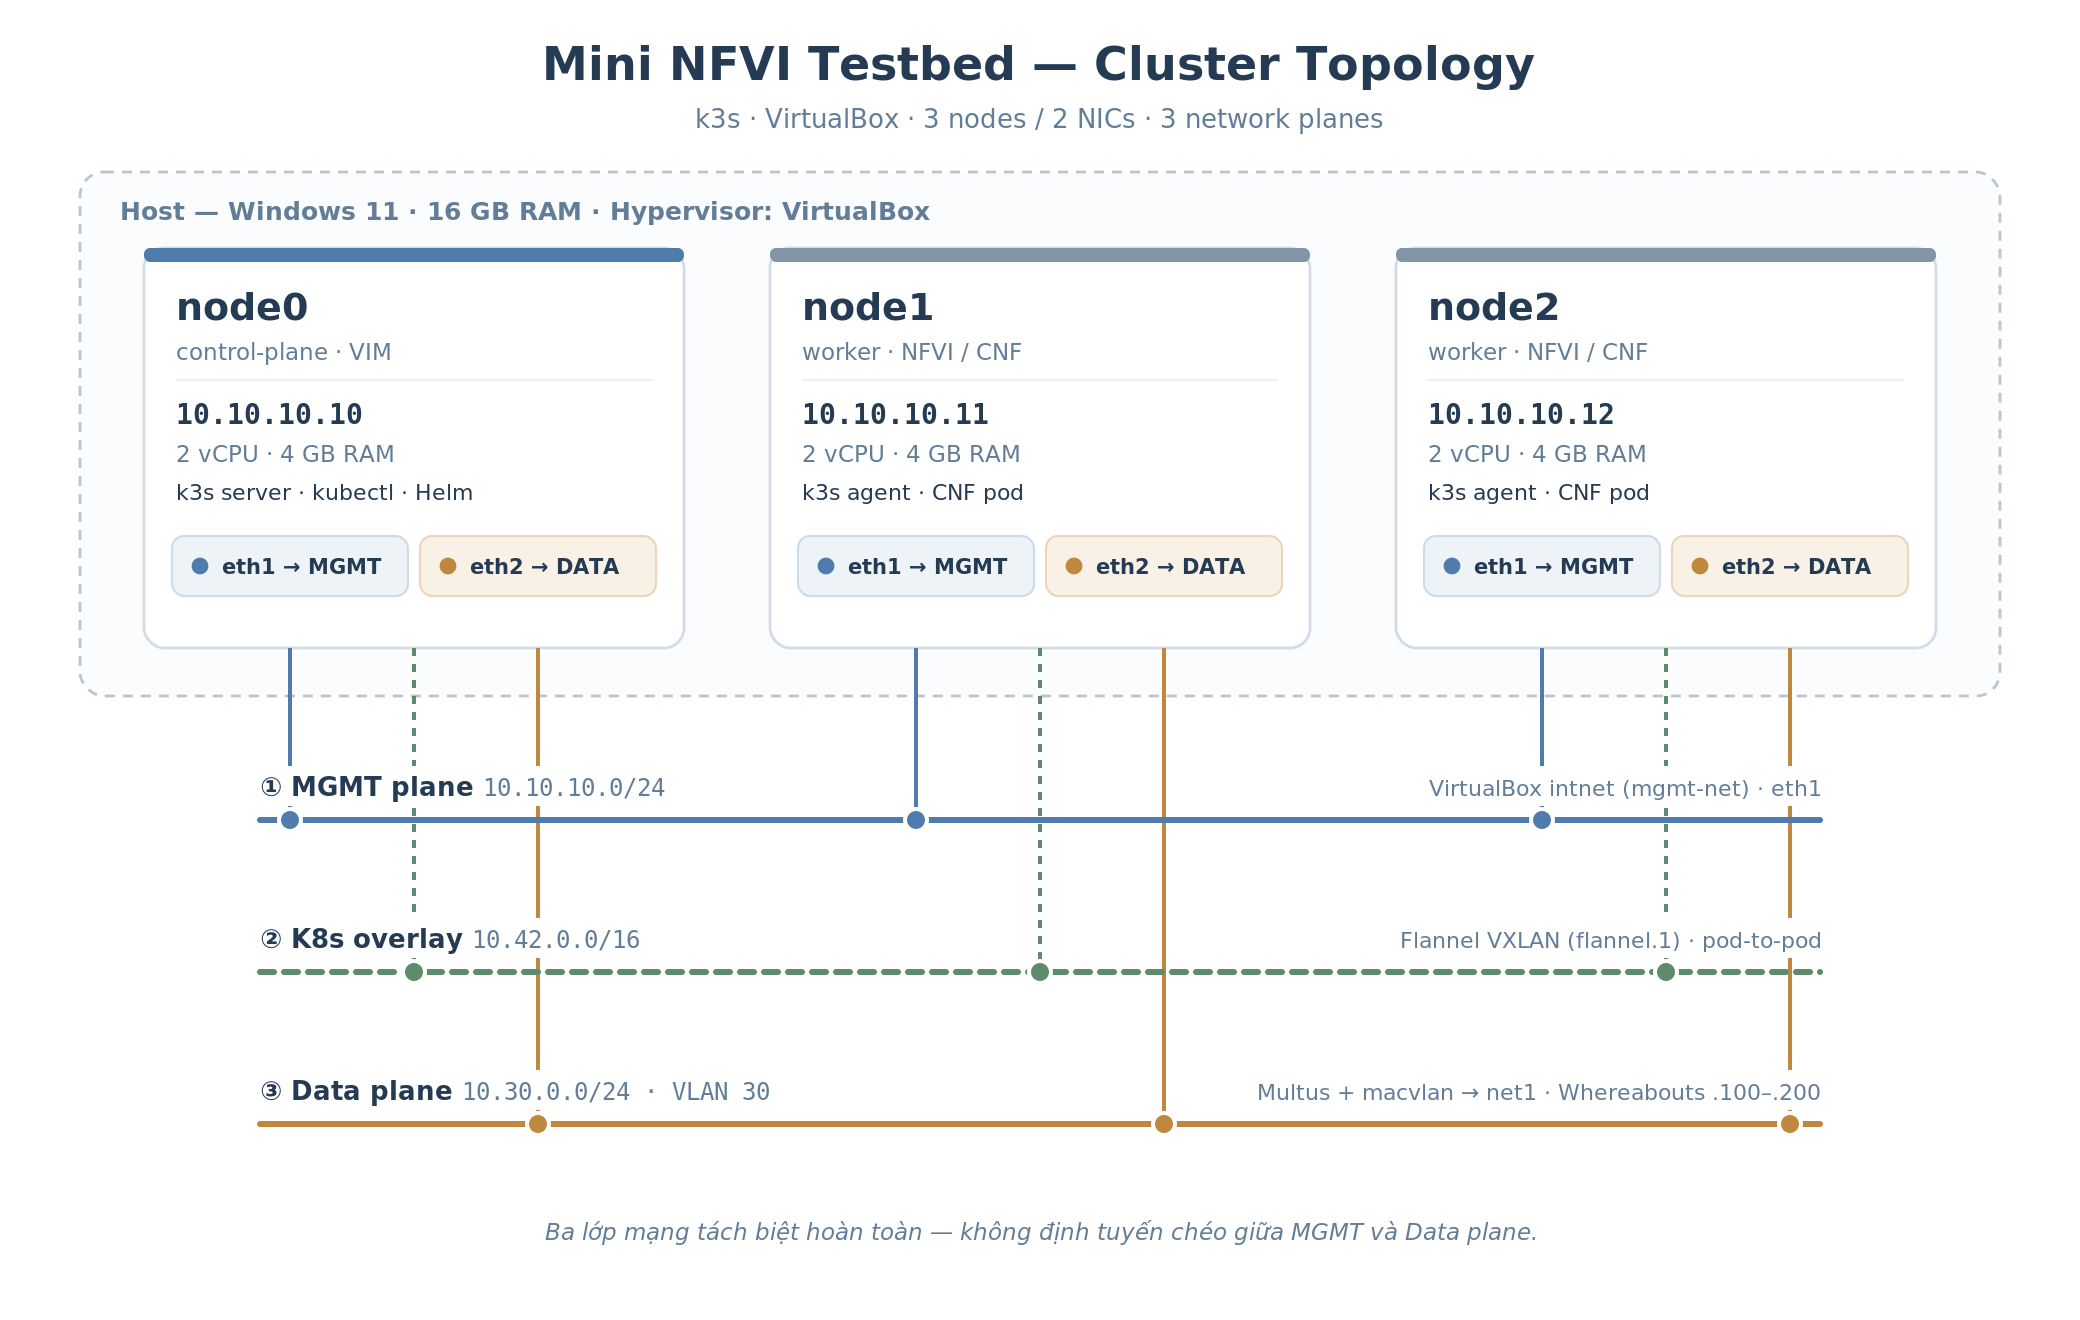
\includegraphics[width=0.9\textwidth]{Images/cluster_topo.png}
    \caption{Three-node cluster topology and dual-interface IP plan.}
    \label{fig:topo}
\end{figure}

\begin{table}[H]
\centering
\begin{tabular}{llll}
\toprule
\textbf{Node} & \textbf{Role} & \textbf{eth1 (MGMT)} & \textbf{eth2 (DATA)} \\
\midrule
node0 & control-plane (k3s server) & 10.10.10.10 & 10.30.0.10 \\
node1 & worker (k3s agent)         & 10.10.10.11 & 10.30.0.11 \\
node2 & worker (k3s agent)         & 10.10.10.12 & 10.30.0.12 \\
\bottomrule
\end{tabular}
\caption{Node roles and per-interface IP addresses.}
\label{tab:nodes}
\end{table}

\subsection{Three-Plane Network Design}

Following telco practice, three logically separate network planes are kept
strictly isolated, as summarised in Table~\ref{tab:planes}.

\begin{table}[H]
\centering
\begin{tabular}{llll}
\toprule
\textbf{Plane} & \textbf{CIDR} & \textbf{Interface} & \textbf{Provider} \\
\midrule
Management    & 10.10.10.0/24 & eth1       & VirtualBox internal net \texttt{mgmt-net} \\
K8s cluster   & 10.42.0.0/16  & flannel.1  & Flannel (VXLAN overlay) \\
Data plane    & 10.30.0.0/24  & eth2 $\rightarrow$ net1 & Multus + macvlan + Whereabouts \\
\bottomrule
\end{tabular}
\caption{The three isolated network planes.}
\label{tab:planes}
\end{table}

\begin{itemize}
    \item The \textbf{management plane} (eth1) carries SSH, the Kubernetes
          API, and telemetry. k3s is explicitly configured so that the node
          IP and control-plane signalling use this interface
          (\texttt{--node-ip}, \texttt{--flannel-iface eth1}).
    \item The \textbf{cluster plane} is the Flannel VXLAN overlay
          (10.42.0.0/16) that provides pod-to-pod connectivity for the
          primary interface \texttt{eth0}.
    \item The \textbf{data plane} (eth2) is dedicated to user-plane traffic.
          Pods receive a second interface \texttt{net1} via macvlan, with IPs
          in the range 10.30.0.100--10.30.0.200 assigned by Whereabouts. No
          routing is configured between the data plane and the other planes,
          enforcing isolation.
\end{itemize}

Because the management and data networks are VirtualBox \emph{internal}
networks, the Windows host has no route into them; Grafana is therefore
reached through an SSH tunnel (Section~5.5).

\subsection{Technology Stack}

\begin{table}[H]
\centering
\begin{tabular}{ll}
\toprule
\textbf{Layer} & \textbf{Technology} \\
\midrule
Hypervisor / IaC       & VirtualBox, Vagrant, Ansible \\
Kubernetes distribution & k3s (embedded datastore) \\
Primary CNI            & Flannel (VXLAN) \\
Secondary CNI          & Multus + macvlan + Whereabouts \\
Package management      & Helm \\
Observability          & kube-prometheus-stack (Prometheus, Grafana, exporters) \\
Auto-scaling           & HorizontalPodAutoscaler + metrics-server \\
Throughput testing     & iperf3 \\
\bottomrule
\end{tabular}
\caption{Technology stack by layer.}
\label{tab:stack}
\end{table}

\subsection{Resource Constraints and Optimisations}

The 16~GB host budget drives several deliberate optimisations:

\begin{itemize}
    \item \textbf{k3s instead of kubeadm} --- a single lightweight binary
          with an embedded datastore avoids the overhead of a full etcd
          control plane.
    \item \textbf{Alertmanager disabled} and \textbf{persistence disabled}
          (\texttt{emptyDir}) in the monitoring stack.
    \item \textbf{Prometheus retention reduced to 2~days} and unused
          scrape targets (etcd, kube-proxy, scheduler) turned off.
    \item \textbf{Grafana exposed via NodePort}, not a LoadBalancer, and
          reached through an SSH tunnel.
    \item \textbf{The thin Multus plugin} is used in preference to the thick
          (daemon-based) variant to minimise the per-node memory footprint.
\end{itemize}
